\begin{figure}
  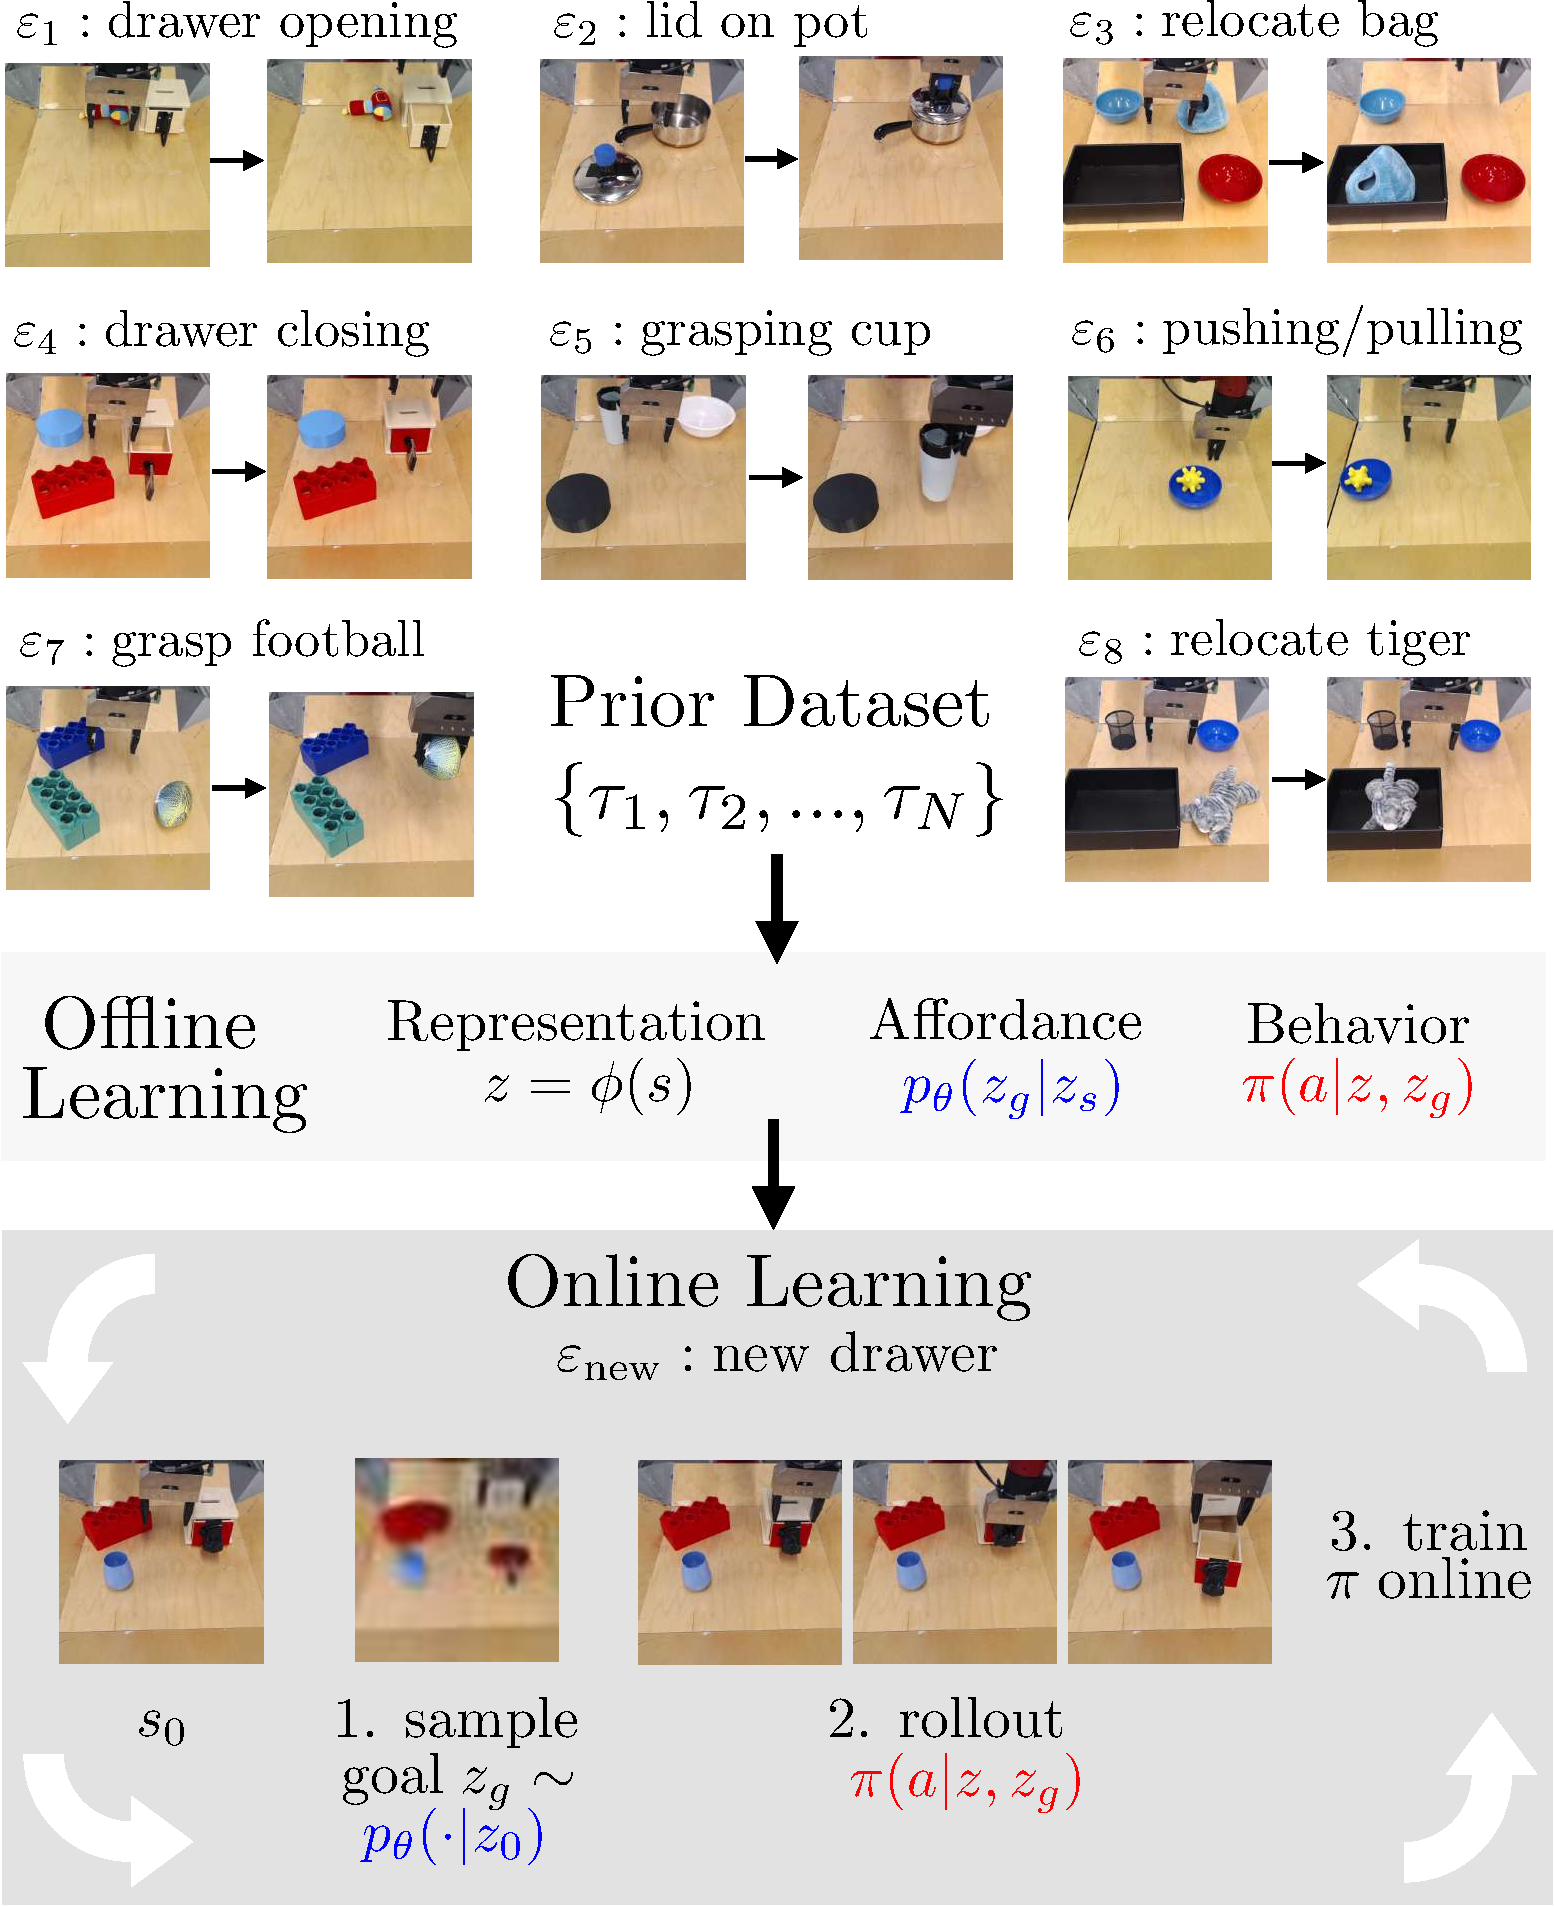
\includegraphics[width=0.99\linewidth]{val/imgs/fig_page1_v8-crop_compressed.pdf}
  \caption{\small
  We propose a system for efficient self-supervised robot learning in an unseen environment $\mathcal{E}_\text{new}$ by utilizing prior data $\mathcal{D}$ of trajectories from related similar environments $\mathcal{E}_i \sim p(\mathcal{E})$. Tasks are specified via a target goal image. From prior data, we learn an encoder $\zt = \phi(\st)$ of images (representation) for compressing observations and self-generating rewards, a model of what tasks might be tested in the new environment (affordance), and goal-conditioned policy to accomplish a given task (behavior). While this provides reasonable performance in some test environments, perfecting the policy in test environments may require additional interaction in the test environment. Dropped in a test environment $\mathcal{E}_\text{new}$ without a given goal, we run RL online in order to practice potential tasks, with goals sampled from the affordance model. Online behavior learning allows us to improve the policy $\pi$ for $\mathcal{E}_\text{new}$ even when it contains new and unseen objects. 
  }
  \label{fig:page1}
  \vspace{-0.5cm}
\end{figure}